\documentclass[12pt,twoside,a4paper]{article}
%-------------------------------------------
%---Packages--------------------------------
%-------------------------------------------
\usepackage[utf8]{inputenc}
%\usepackage[T1]{fontenc}
%\usepackage{txfonts}
\usepackage{amsmath}
\usepackage{amsthm}
\usepackage{amsfonts}
\usepackage{array}
\usepackage{amssymb}
\usepackage{blindtext}
\usepackage{caption}
\usepackage{color}
\usepackage{csquotes}	    %
\usepackage{enumitem}	    %pour mieux bosser avec les listes. ajoute option label
\usepackage[yyyymmdd]{datetime}        %pour définir date custom
\usepackage{etaremune}
\usepackage{environ}
\usepackage{fancybox}
\usepackage{fancyhdr} 	    % Custom headers and footers
\usepackage{fancyref}
%\usepackage{float}
\usepackage{floatrow}       %float and floatrow can't be together...
\usepackage{gensymb}
\usepackage{graphicx}
\usepackage[colorlinks=true, linkcolor=purple, citecolor=cyan]{hyperref}
\usepackage{footnotebackref}
\usepackage{lipsum}
\usepackage{mathtools}
\usepackage{multicol}	    %gérer plusieurs colonnes
\usepackage{setspace}
\usepackage{subcaption}
\usepackage{todonotes}	    %Bonne gestion des TODOs
%TODO commenté pour tester l'utilité... à voir% \usepackage[tc]{titlepic}      %Permet de mettre une image en page de garde
\usepackage{tikz}	    % Pour outil de dessin puissant
\usepackage{ulem}	    %underline sur plusieurs lignes (avec \uline{})
\usepackage{vmargin} 	    %gestion des marges, avec dans l'ordre : gauche, haut, droit, bas, en-tête, entre en-tête et texte, bas de page, hauteur entre bas de page et texte
\usepackage{wrapfig}
\usepackage{xcolor}
\usepackage{xparse}                    %Pour utiliser NewDocumentCommand et des arguments 'mmooo'
%\usepackage{fullpage} 	    %supprime toutes les marges allouées aux notes, aussi en haut et en bas

%\ExplSyntaxOn
\pagestyle{fancyplain}	    %Makes all pages in the document conform to the custom headers and footers

%-------------------------------------------
%---Document Commands-----------------------
%---------------------------{----------------
\NewDocumentCommand{\framecolorbox}{oommm}
 {% #1 = width (optional)
  % #2 = inner alignment (optional)
  % #3 = frame color
  % #4 = background color
  % #5 = text
  \IfValueTF{#1}%
   {\IfValueTF{#2}%
    {\fcolorbox{#3}{#4}{\makebox[#1][#2]{#5}}}%
    {\fcolorbox{#3}{#4}{\makebox[#1]{#5}}}%
   }%
   {\fcolorbox{#3}{#4}{#5}}%
 }%
%------------------------------------------------
%------------------ENGLISH----------------------
%----------------------------------------------

\NewDocumentCommand{\epflTitle}{mO{Olivier Cloux}O{\today}O{Notes de Cours en}D<>{../../Common}}%Arguments : Matière, Auteur, Date, Titre du doc
{
\begin{titlepage}
    \vspace*{\fill}
    \begin{center}
        \normalfont \normalsize
        \textsc{Ecole Polytechnique Fédérale de Lausanne} \\ [25pt] % Your university, school and/or department name(s)
        \textsc{#4} %Titre du doc
        \\ [0.4 pt]
        \horrule{0.5pt} \\[0.4cm] % Thin top horizontal rule
        \huge #1 \\ % Matière
        \horrule{2pt} \\[0.5cm] % Thick bottom horizontal rule
        
\includegraphics[width=8cm]{#5/EPFL_logo}
        ~\\[0.5 cm]
        \small\textsc{#2}\\[0.4cm]
        \small\textsc{#3}\\
        ~\\
        ~\\
        
\includegraphics[scale=0.5]{#5/creativeCommons}
    \end{center}
    \vspace*{\fill}
\end{titlepage}
}


%-------------------------------------------
%-------------MATH NEW COMMANDS-------------
%-------------------------------------------
\newcommand{\somme}[2]{\ensuremath{\sum\limits_{#2}^{#1}}}
\newcommand{\produit}[2]{\ensuremath{\prod\limits_{#2}^{#1}}}
\newcommand{\limite}{\lim\limits_}
\newcommand{\llimite}[3]{\limite{\substack{#1 \\ #2}}\left(#3\right)}	%limites à deux condiitons
\newcommand{\et}{\mbox{ et }}
\newcommand{\deriv}[1]{\ensuremath{\, \mathrm d #1}}	%sigle dx, dt,dy... des dérivées/intégrales
%\newcommand{\fx}{\ensuremath{f'(\textbf{x}_0 + h}}
\newcommand{\ninf}{\ensuremath{n \to \infty}}	       %pour les limites : n tend vers l'infini
\newcommand{\xinf}{\ensuremath{x \to \infty}}	       %pour les limites : x tend vers l'infini
\newcommand{\infint}{\ensuremath{\int_{-\infty}^{\infty}}}
\newcommand{\xo}{\ensuremath{x \to 0}}									%x to 0
\newcommand{\no}{\ensuremath{n \to 0}}									%n zéro
\newcommand{\xx}{\ensuremath{x \to x}}									%x to x
\newcommand{\Xo}{\ensuremath{x_0}}										%x zéro
\newcommand{\X}{\ensuremath{\mathbf{X}} }
\newcommand{\A}{\ensuremath{\mathbf{A}} }
\newcommand{\R}{\ensuremath{\mathbb{R}} }								%ensemble de R
\newcommand{\rn}{\ensuremath{\mathbb{R}^n} } 							%ensemble de R de taille n
\newcommand{\Rm}{\ensuremath{\mathbb{R}^m} }  							%ensemble de R de taille m
\newcommand{\C}{\ensuremath{\mathbb{C}} }
\newcommand{\N}{\ensuremath{\mathbb{N}} }
\newcommand{\Z}{\ensuremath{\mathbb{Z}} }
\newcommand{\Q}{\ensuremath{\mathbb{Q}} }
\newcommand{\rtor}{\ensuremath{\R \to \R} }
\newcommand{\pour}{\mbox{ pour }}
\newcommand{\coss}[1]{\ensuremath{\cos\(#1\)}}						%cosinus avec des parenthèses de bonne taille (genre frac)
\newcommand{\sinn}[1]{\ensuremath{\sin\(#1\)}}					%sinus avec des parentèses de bonne taille (genre frac)
\newcommand{\txtfrac}[2]{\ensuremath{\frac{\text{#1}}{\text{#2}}}}		%Fractions composées de texte
\newcommand{\evalfrac}[3]{\ensuremath{\left.\frac{#1}{#2}\right|_{#3}}}
\renewcommand{\(}{\left(}												%Parenthèse gauche de taille adaptive
\renewcommand{\)}{\right)}
\newcommand{\longeq}{=\joinrel=}												%Parenthèse droite de taille adaptive


%-------------------------------------------------------
%------------------MISC NEW COMMANDS--------------------
%-------------------------------------------------------
\newcommand{\degre}{\ensuremath{^\circ}}
%\newdateformat{\eudate}{\THEYEAR-\twodigit{\THEMONTH}-\twodigit{\THEDAY}}



%-------------------------------------------------------
%------------------TEXT NEW COMMANDS--------------------
%-------------------------------------------------------
\newcommand{\ts}{\textsuperscript}
\newcommand{\evid}[1]{\textbf{\uline{#1}}}        %mise en évidence (gras + souligné)



%\newcommand{\Exemple}{\underline{Exemple}}
\newcommand{\Theoreme}{\underline{Théorème}}
\newcommand{\Remarque}{\underline{Remarque}}
\newcommand{\Definition}{\underline{Définition} }
\newcommand{\skinf}{\sum^{\infty}_{k=0}}
\newcommand{\combi}[2]{\ensuremath{\begin{pmatrix} #1 \\ #2 \end{pmatrix}}}	%combinaison parmi 1 de 2
\newcommand{\intx}[3]{\ensuremath{\int_{#1}^{#2} #3 \deriv{x}}}				%intégrale dx
\newcommand{\intt}[3]{\ensuremath{\int_{#1}^{#2} #3 \deriv{t}}}				%intégrale dy
\newcommand{\misenforme}{\begin{center} Mis en forme jusqu'ici\\ \line(1,0){400}\\ normalement juste, mais à améliorer depuis ici\end{center}}	%raccourci pour mise en forme
\newcommand*\circled[1]{\tikz[baseline=(char.base)]{
            \node[shape=circle,draw,inner sep=1pt] (char) {#1};}}			%pour entourer un chiffre
\newcommand{\horrule}[1]{\rule{\linewidth}{#1}} 				% Create horizontal rule command with 1 argument of height

\theoremstyle{definition}
\newtheorem{exemp}{Exemple}
\newtheorem{examp}{Example}


%-------------------------------------------
%---Environments----------------------------
%-------------------------------------------
\NewEnviron{boite}[1][0.9]{%
	\begin{center}
		\framecolorbox{red}{white}{%
			\begin{minipage}{#1\textwidth}
 	 			\BODY
			\end{minipage}
		}
	\end{center}
}
\NewEnviron{blackbox}[1][0.9]{%
	\begin{center}
		\framecolorbox{black}{white}{%
			\begin{minipage}{#1\textwidth}
 	 			\BODY
			\end{minipage}
		}
	\end{center}
}
\NewEnviron{exemple}[1][0.8]{%
    \begin{center}
        \framecolorbox{white}{gray!20}{%
            \begin{minipage}{#1\textwidth}
                \begin{exemp}
                    \BODY
                \end{exemp}
            \end{minipage}
        }
    \end{center}
}
\NewEnviron{suiteExemple}[1][0.8]{%
    \begin{center}
        \framecolorbox{white}{gray!20}{%
            \begin{minipage}{#1\textwidth}
                \BODY
            \end{minipage}
        }
    \end{center}
}
\NewEnviron{colExemple}[1][0.8]{%
    \begin{center}
        \framecolorbox{white}{gray!20}{%
            \begin{minipage}{#1\columnwidth}
                \begin{exemp}
                    \BODY
                \end{exemp}
            \end{minipage}
        }
    \end{center}
}
\NewEnviron{example}[1][0.8]{%
    \begin{center}
        \framecolorbox{white}{gray!20}{%
            \begin{minipage}{#1\textwidth}
                \begin{examp}
                    \BODY
                \end{examp}
            \end{minipage}
	}
    \end{center}
}
\NewEnviron{systeq}[1][l]{
			\begin{center}
				$\left\{\begin{array}{#1}
					\BODY
				\end{array}\right.$
			\end{center}
 }





%-------------------------------------------
%---General settings-----------------------
%-------------------------------------------
\renewcommand{\headrulewidth}{1pt}										%ligne au haut de chaque page
\renewcommand{\footrulewidth}{1pt}										%ligne au pied de chaque page
\setstretch{1.6}
\author{Olivier Cloux}

%\usepackage{algorithmicx}
\usepackage{algorithm}
\usepackage{algorithmic}
\usepackage[tc]{titlepic}
\usepackage{graphicx}
\usepackage{blindtext}
\usepackage[toc,page]{appendix}
%\usepackage[a4paper]{geometry}
%\setcounter{section}{-1}
\renewcommand{\contentsname}{Table des Matières}
\begin{document}
\epflTitle{Algorithms I}[Olivier Cloux][Fall 2015][Lectures notes in]	%Chose \epflTitleEN{#1}[#2][#3] #1 mand. : course's name, #2 opt. : name, #3 opt. : Date
\setstretch{1}
\tableofcontents
\setstretch{1.2}
\section{Sorting}
\subsection{Insertion Sort}
The idea : Start with an empty array, and add an element at the end : if it is smaller than it's left neighbour, swap them ; repeat this last operation until left neighbour is smaller or equal.

With that, our hand is always sorted. The algorithm is :
\begin{algorithm}
	\caption{\texttt{Insertion-Sort}$(A,n)$}
	\begin{algorithmic}
		\FOR{$j=2$ \textbf{to} $n$}
			\STATE $key = A[j]$
			\STATE \textit{//insert A[j] into the sorted sequence A[1...j-1].}
			\STATE $i = j-1$
			\WHILE{$i > 0$ \textbf{and} $A[i] > key$}
				\STATE $A[i+1] = A[i]$
				\STATE $i = i-1$
			\ENDWHILE
			\STATE $A[i+1] = key$
		\ENDFOR
	\end{algorithmic}
\end{algorithm}
Furthermore, as we don't require more space to solve it, we say that the algorithm is \textbf{in-place}
To prove it, our loop invariant is : \paragraph{At the start of the "outer" for loop (the loop indexed by j), the subarray A[1...j-1] consists of the elements originally in A[1...j-1] but in sorted order.}
\subsection{Loop Invariant}
A loop invariant is a statement that is satisfied during the loop. It must verify 3 points :
\begin{itemize}
	\item 	\textbf{Initialization}: it is true prior to the first iteration of the loop.
	\item 	\textbf{Maintenance}: if it is true before an iteration of the loop, it remains true before next iteration.
	\item 	\textbf{Termination}: when the loop terminates, the invariant (usually along with the reason the loop terminated) gives us a useful property that helps show that the algorithm is correct
\end{itemize}
\subsection{Divide and Conquer : Merge sort}
\begin{wrapfigure}{r}{7cm}
	\centering
	\captionsetup{justification=centering}	
	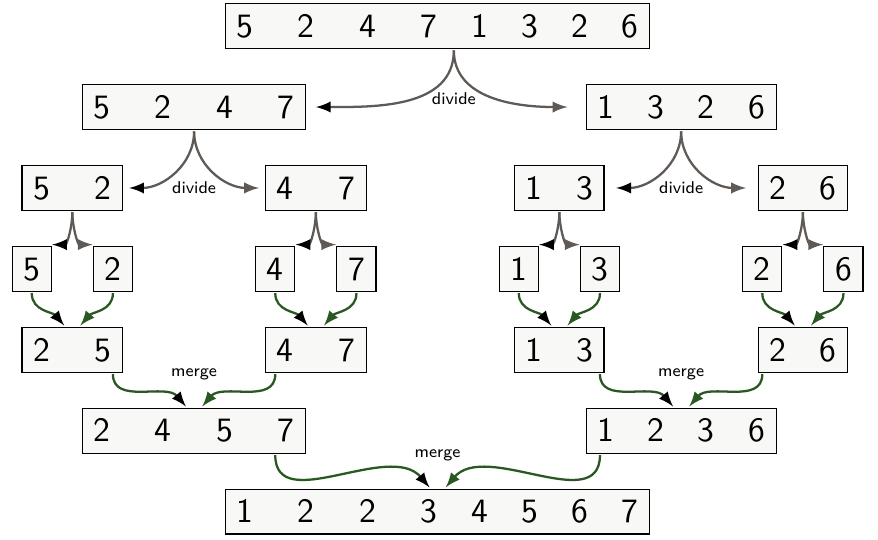
\includegraphics[scale=0.3]{images/mergeSort}
	\caption{Merge-Sort on \{5,2,4,7,1,3,2,6\}}
\end{wrapfigure}
Use 3 simple but powerful steps : \textbf{Divide} (the problem into a number of sub-problems that are smaller instances of the same problem), \textbf{conquer} (the sub-problems by solving them recursively)\footnote{Base case : If the sub-problems are small enough, just solve them by brute force} , \textbf{combine} (the sub-problem solutions to give a solution to the original problem)

The algorithm is quite simple : we split into 2 sub-problems (recursively) and then merge them. :
\begin{algorithm}
	\caption{\texttt{Merge-Sort}$(A,p,r)$}
	\begin{algorithmic}
		\IF{$p<r$}
			\STATE 	$q = \lfloor\(\frac{p+r}{2}\)\rfloor \quad$ 
			\STATE 	\texttt{Merge-Sort}$(A,p,q)$
			\STATE	\texttt{Merge-Sort}$(A,q+1,r)$
			\STATE	\texttt{Merge}$(a,p,q,r)$
		\ENDIF
	\end{algorithmic}
\end{algorithm}
\begin{boite}[0.6]
	 \centering
	 This one runs in $\Theta(l\log(n)$. See later for proof.
\end{boite}
But once we divided (q = ...) and conquered (recursive call to \texttt{Merge-Sort}), we still have to combine (with \texttt{Merge}). The idea behind this this algorithm is slightly different : \\
\textbf{Input :} An array A and indices $p \leq q \leq r$ such that sub-arrays $A[p...q]$ and $A[q+1...r]$ are sorted\\
\textbf{Output :} The two sub-arrays are merged into a single sorted array $A[p...r]$ 
\begin{algorithm}
	\caption{\texttt{Merge}$(A,p,q,r)$}
	\begin{algorithmic}
		\STATE $n_1 = q-p+1\ ; \ n_2 = r-q$
		\STATE Let $L[1...n_1+1]$ and $R[1...n_2+1]$ be new arrays
		\FOR{$i = 1$ \textbf{to} $n_1$}
			\STATE $L[i] = A[p+i-1]$
		\ENDFOR
		\FOR{$j=1$ \textbf{to} $n_2$}
			\STATE $R[j] = A[q+j]$
		\ENDFOR
		\STATE $L[n_1+1] = \infty\ ; \ R[n_2+1] = \infty\ ;\ i=1\ ;\  j=1$
		\FOR{$k=p$ \textbf{to} $r$}
			\IF{$L[i] \leq R[j]$}
				\STATE $A[k] = L[i]$
				\STATE $i = i+1$
			\ELSE
				\STATE $A[k] = R[j]$
				\STATE $j = j+1$
			\ENDIF
		\ENDFOR
	\end{algorithmic}
\end{algorithm}
\begin{boite}[0.4]
	\centering
	This one runs in $\Theta(n)$
\end{boite}
Sadly, as the algorithm needs to create other arrays, we say that \textbf{it is not in-place}.
\subsection{Solving recurrences}
This is our first recurrent algorithm (meaning we call it on similar sub-problems, requiring us to continue the algorithm (use \texttt{Merge}) but on multiple level.  To analyse the running time of this kind of algorithm, we define $T(n)$ as the running time of a problem of size n. If $n$ is small enough, say $n \leq c$ for some constant $c$, then $T(n) = \Theta(1)$. Otherwise, we divide our problem into \textit{a} problems, each of size \textit{b}.  We also need to compute $D(n)$ the time to divide and $C(n)$ the time to combine. Thus, we get the recurrence :
\begin{equation}
T(n) = \left\{\begin{array}{ll}
	\Theta(1) & n\leq c\\
	aT(n/b) + D(n) + C(n) &  \text{Otherwise}
\end{array}\right.
\end{equation}
In our precise case, $D(n) = \Theta(1)$ as it takes constant time. Combine, takes $\Theta(n)$, as seen earlier. Finally, the Conquer part gives us two subproblems, each of size $n/2 \to 2T(n/2)$. Combining all this, we want to solve the recurrence :
\[T(n) = \left\{\begin{array}{ll}
c & \text{if } n=1\\
2T\(\frac{n}{2}\) + \Theta(n) + \Theta(1)& \text{otherwise}
\end{array}\right.\]
To solve recurrence, we have 3 techniques :
\setstretch{1}
\begin{itemize}
	\item 	Substitution method
	\item 	Recursion tree
	\item 	Master Method
\end{itemize}
\setstretch{1.2}
\subsubsection{Substitution method}
We have to guess the form of the solution, and then use mathematical induction to find the constants and show that the solution works.\\
\begin{exemple}
	\[\begin{array}{rl}
	T(n) &= 2T(n/2) + c\cdot n\\
	&= 2(2T(n/4) + c\cdot n/2) + c\cdot n = 4T(n/4) + 2\cdot cn\\
	&= 4(2T(n/8) + c\cdot n/4) + 2\cdot bn = 8T(n/8) + 3\cdot cn\\
	&\vdots\\
	&= 2^kT(n/2^k) + k\cdot cn
	\end{array}\]
	We can make a guess : $T(n) =  \Theta\big(n\log(n)\big)$. In order to prove that, we have to prove the upper bound ---$T(n) = O\big(n\log(n)\big)$--- and then the lower bound ---$\Omega\big(n\log(n)\big)$---. For the proof, see Appendix \ref{appendix: substitution method}.
\end{exemple}

\subsubsection{Recursion tree}
\begin{wrapfigure}{r}{8cm}
	\centering
	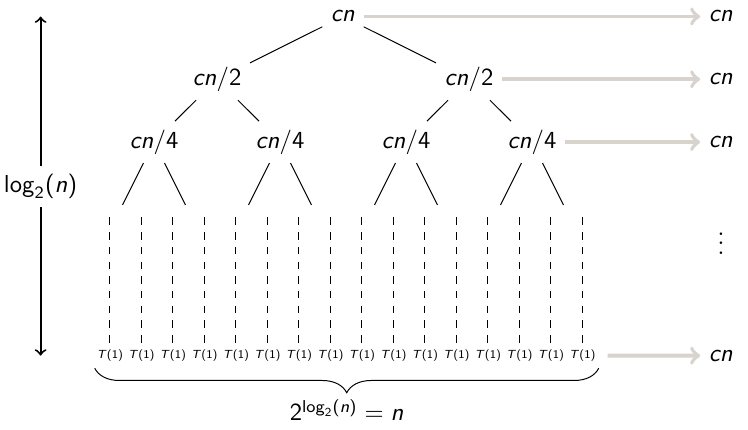
\includegraphics[scale=0.5]{images/recursion_Tree}
	\captionsetup{justification=centering}
	\caption{The recursion tree of our favourite example}
	\label{fig: recursion tree}
\end{wrapfigure}
Recursion tree is useful to generate a guess. It does not hold for a formal proof. Once the guess is generated, we still have to verify by substitution method. Each node corresponds to the cost of a subproblem. We sum the costs within each level of the tree to obtain a set of per-level costs, then we sum all the per-level costs to determine the total cost of all levels of the recursion. With the tree in Figure \ref{fig: recursion tree}, we can make a qualified guess : $T(n) = cn\log_2n = \Theta(n \log n)$
\begin{figure}[h]
	\centering
	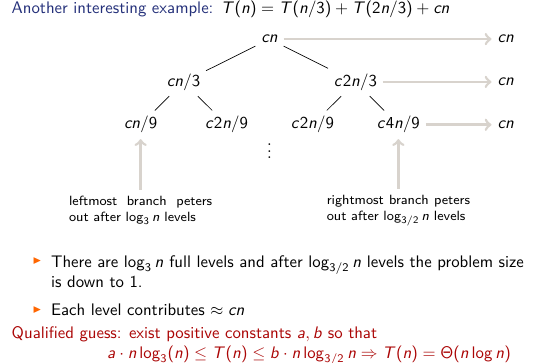
\includegraphics[scale=0.7]{images/interesting_example_recursion_tree}
	\caption{An other recursion tree}
	\label{fig: interesting example recursion tree}
\end{figure}
~
\subsubsection{Master Theorem}
The idea here is to solve recurrences of the form $T(n) = a T(n/b) + f(n)$. Comprehensive way : look at complexity of both terms ($aT(n/b)$ and $f(n)$). For the last it easy, it usually already is in the form $\Theta(...)$. For the first, compute \uline{$n^{\log_b(a)}$}
If it it greater than complexity of $f(n)$, this is the complexity, if $f(n)$ is greater then use $f(n)'s$ complexity. Subtlety : if they are equal, then return $n^{\log_b(a)} \cdot \log n$
\begin{exemple}
	Recall the favourite example : $T(n) = 2T(n/2) + cn,\ T(1) = c$. We immediately see that $f(n) = O(n)$, and, using $a = b = 2 \to n^{\log_{2}(2)} = n^1 = n$ ; as the two are equals, we have 
	\[T(n) = \Theta(n^{\log_2(2)} \log n) = \Theta(n \log n)\]
\end{exemple}
\begin{exemple}
	Now, consider a slightly different recursion :
	\[T(n) = 2T(n/2) + c\]
	As before, we have $a = b = 2 \to n^{\log_{2}(2)} = n^1 = n$. But now, $f(n) = O(1)$. We pick the greatest complexity (because it dominates the analysis), giving us 
	\[T(n) = \Theta(n)\]
\end{exemple}


\section{Maximum-subarray problem}
For that, we get as an input an array of numbers $A[1...n]$. We must find indices $i$ and $j$ such that $A[i...j]$ has the greatest sum of any subarray of A. 

The first natural way to do it is to test all combinations, like 2 nested for-loop (i from 1 to n, j from i to n), we store a temporary value and a "current best" to be compared with temp. it works, but in $\Theta(n^2)$ with space $\Theta(n)$

\begin{wrapfigure}{r}{7cm}
	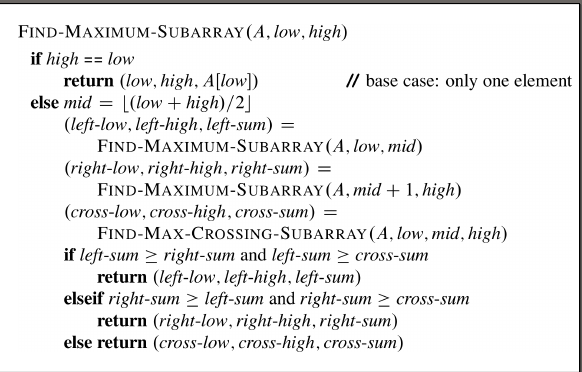
\includegraphics[scale=0.7]{images/find_max_subarray}
\end{wrapfigure}
A better algorithm uses Divide-and-Conquer on the array, and (using recursion) find the best sum in the subarrays. It works, but this solution does not consider solutions crossing the mid point. Our strategy must cover the 3 cases : either the best subarray is in the left part, or in the right part, or crossing the mid point. Our "divide-and-conquer" has the following steps : Divide (into 2 sub problems of approximately equal size), conquer (by finding best subarray in both side, recursively), and finally combine (by finding a maximum solution that crosses the mid point, and using the best solution out of the three).

In order to find the best crossing subarray, we use the idea that, considering only a side, the subarray is also the best in this part \uline{beginning from the middle}. So, given 2 arrays, we start at the middle (end of left and beginning of right), and go through each part until all left and all right is visited. The best crossing subarray consists of the best in left with best in right.		

The recurrence of this search is 
\[T(n) = \left\{\begin{array}{ll}
	\Theta(1) & \text{if } n=1\\
	2T(n/2) + \Theta(n) & \text{otherwise}
\end{array}\right.\]
A tight analysis (for example using master method), returns :
\begin{boite}[0.4]
	\[T(n) = \Theta(n \log n)\]
\end{boite}

\section{Matrix multiplication}
A small subject, for comprehension. You are given A,B, two $n\times n$ matrix and want to output their product. The algorithm use by humans, multiplying the x\ts{th} line of A by the x\ts{th} column of B, is really inefficient as it uses 3 nested for-loops each of size n, resulting in a $\Theta{n^3}$ running time for a $\Theta{n^2}$ space. Even using a divide and conquer algorithm (separating matrix in smaller square matrix) is as complicated : separating in each matrix in 4 $n/2$ square matrix will still result in 8 multiplications $A_{11}B_{11} + A_{12}B_{21}\ldots$. We can prove the complexity is $\Theta(n^{log_2(8)} = \Theta(n^3)$

Here, the best solution is by using \textbf{Strassen's algorithm}. By some mathematical subtlety, we do the same computation but using only 7 multiplications (even with several more additions, but just a constant more). This algorithm runs in
\begin{boite}[0.4]
	\[T(n) = \Theta\(n^{\log_2(7)}\)\]
\end{boite}
The algorithm is the following :
	\begin{itemize}
		\item 	\textbf{Divide }each matrix in 4 $n/2 \times n/2$ square matrix.
				\[\begin{pmatrix}
					C_{11} & C_{12}\\
					C_{21} & C_{22}
				\end{pmatrix} 
				= 
				\begin{pmatrix}
					A_{11} & A_{12}\\
					A_{21} & A_{22}
				\end{pmatrix} 
				\cdot 
				\begin{pmatrix}
					B_{11} & B_{12}\\
					B_{21} & B_{22}
				\end{pmatrix}\]
		\item 	\textbf{Conquer :} Calculate the following 7 multiplications :
				\begin{multicols}{2}
					\begin{itemize}
						\item 	$M_1 := (A_{11} + A_{22})(B_{11} + B_{22})$
						\item 	$M_2 := (A_{21} + A_{22})B_{11}$
						\item 	$M_3 := A_{11}(B_{12}-B_{22})$
						\item 	$M_4 := A_{22}(B_{21}-B_{11})$
						\item 	$M_5 := (A_{11} + A_{12})B_{22}$
						\item 	$M_6 := (A_{21}  A_{11})(B_{11}+B_{12})$
						\item 	$M_7 := (A_{12} - A_{22})(B_{21}+B_{22})$
					\end{itemize}
				\end{multicols}
		\item 	\textbf{Combine :} let :
				\begin{multicols}{2}
					\begin{itemize}
						\item 	$C_{11} = M_1 + M_4 - M_5 + M_7$
						\item	$C_{21} = M_2 + M_4$
						\item 	$C_{12} = M_3 + M_5$
						\item 	$C_{22} = M_1 - M_2 + M_3 + M_6$
					\end{itemize}
				\end{multicols}
	\end{itemize}
\section{Heap Sort}
\begin{wrapfigure}{r}{6cm}
	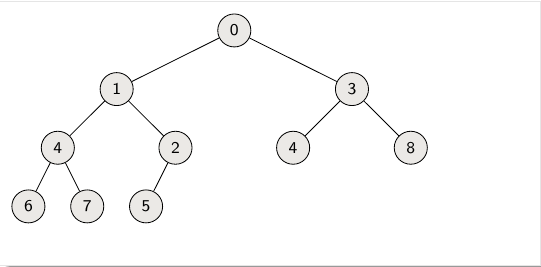
\includegraphics[scale=0.6]{images/minHeap}
\end{wrapfigure}
Heap data structures, are a binary tree. From a node, the 2 children (both elements under him) are greater to this node (min-heap) or smaller (max-heap). So, in a \textit{max heap}, the maximum element is the root. In a \textit{min heap}, the minimum element is the root.We define the height of a node as the longest simple path from the node down to a leaf, and the height of heap as the height of root ($\Theta(\log n)$)

\subsection{Storage}
\begin{figure}[h!]
	\centering
	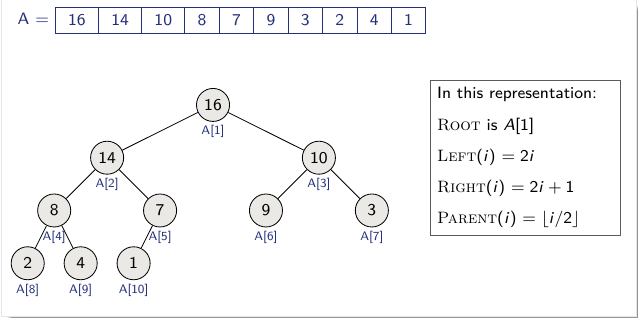
\includegraphics[scale=1]{images/buildHeap}
\end{figure}
We place the elements of our tree in an array. Let's note that, given an array, we can easily find the linked tree. From an element $A[i]$, the the left children is at $A[2i]$ and right children is at $A[2i+1]$. Inversely, the parent of a given node is at $A[\lfloor i/2 \rfloor]$

\subsection{Procedures}
We will use a few algorithms, in order to manipulate these heaps :
\subsubsection{\texttt{Max-Heapify}}
\begin{algorithm}
	\caption{\texttt{Max-Heapify}(A,i,n)}
	\begin{algorithmic}
		\STATE l = LEFT(i)
		\STATE r = RIGHT(i)
		\IF{l $\leq$ n and A[l] > A[i]}
			\STATE largest = l
		\ELSE
			\STATE largest = i
		\ENDIF
		\IF{r $\leq n$ and A[r] > A[largest]}
			\STATE largest = r
		\ENDIF
		\IF{largest $\neq$ i}
			\STATE exchange A[i] with A[largest]
			\STATE \texttt{Max-Heapify}(A,largest,n)
		\ENDIF
	\end{algorithmic}
\end{algorithm}
In other words : we take the elements one after the other and exchange it with the largest of it's two children. Apply until the two children are smaller than the considered element. Apply for all the elements.
\begin{boite}[0.5]
	\centering
	Runs in $\Theta($height of $i) = O(\log n)$\\
	Space = $\Theta(n)$
\end{boite}
\subsubsection{\texttt{Build-Max-Heap}}
This one is quit simple : we start from the bottom, i.e. we don't "sort" the leafs, as they are root of trivially sorted trees. Thus, we start at $\lfloor n/2 \rfloor$ downto 1, and apply \texttt{Max-Heapify} on every of those sub-trees. Here is the code :
\begin{algorithm}
	\caption{\texttt{Build-Max-Heap}}
	\begin{algorithmic}
		\FOR{$i = \lfloor n/2 \rfloor$ \textbf{downto} 1}
			\STATE \texttt{Max-Heapify}(A,i,n)
		\ENDFOR
	\end{algorithmic}
\end{algorithm}
And for the runtime : we will do $O(n)$ calls to \texttt{Max-Heapify}, (actually n/2, but a constant away from n), and each call will take $O(n\log n)$ (as seen previously). Thus :
\begin{boite}[0.4]
	\centering
	Runs in $O(n\log n)$
\end{boite}
\subsubsection{\texttt{HeapSort}}
The idea is to first build the max heap, then, as long as not everything is sorted, exchange the root (biggest element) and the last one of the array (thus one of the smallest). We will then heapify the given tree, of size n-1 (we don't touch the last element, now the biggest). By recursion, we will sort the array. The code is :
\begin{algorithm}
	\caption{\texttt{Heapsort}(A,n)}
	\begin{algorithmic}
		\FOR{$i=n$ \textbf{downto} 2}
			\STATE exchange A[1] with A[i]
			\STATE \texttt{Max-Heapify}(A,1,i-1)
		\ENDFOR
	\end{algorithmic}
\end{algorithm}
			
	

\subsection{Heap implementation of priority queue}
\subsubsection{Increase }

\section{Elementary Data structures}
\subsection{Stacks (LIFO)}
We have 2 operations : \texttt{PUSH(S,x)} (add an element x on the stack S) and \texttt{POP(S)} (take the element of S)

\subsection{Queues (FIFO)}
Exactly what happens with a queue (in a store,...). Elements are pushed at the end, and dequeuing an element will give back the oldest (first who came in)
\subsection{Linked List}
(Double) Linked lists are a dynamic data structure without a predefined size. It's really easy to insert or delete an element, but search is quite long. 
\subsubsection{Searching}
\begin{algorithm}
	\caption{\texttt{List-Search}$(L,k)$}
	\begin{algorithmic}
		\STATE x  $\leftarrow$ L.head
		\WHILE {x $\neq$ nil and x.key $\neq$ k}
			\STATE x $\leftarrow$ x.next
		\ENDWHILE
		\RETURN x
	\end{algorithmic}
\end{algorithm}

\begin{boite}[0.5]
	\centering
	This algorithm has a complexity $\Theta(n)$
\end{boite}

\subsubsection{Inserting}
\begin{algorithm}
	\caption{\texttt{List-Insert}(L,x)}
	\begin{algorithmic}
		\STATE x.next $\leftarrow$ L.head
		\IF{L.head $\neq$ nil}
			\STATE L.head.prev $\leftarrow$ x
		\ENDIF
		\STATE L.head $\leftarrow$ x
		\STATE x.prev = NIL
	\end{algorithmic}
\end{algorithm}

\begin{boite}[0.5]
	\centering
	This algorithm has a complexity $\Theta(1)$
\end{boite}
\newpage
\subsubsection{Deleting}
\begin{algorithm}
	\caption{\texttt{List-Delete}(L,x)}
	\begin{algorithmic}
		\IF{x.prev $\neq$ nil}
			\STATE x.prev.next $\leftarrow$ x.next
		\ELSE 
			\STATE L.head $\leftarrow$ x.next
		\ENDIF
		\IF{x.next $\neq$ nil}
			\STATE x.next.prev $\leftarrow$ x.prev
		\ENDIF
	\end{algorithmic}
\end{algorithm}
\begin{boite}[0.5]
	\centering
	This algorithm has a complexity $\Theta(1)$
\end{boite}

\section{Binary search tree}
In this structure, it is harder to insert or delete an element than in a linked list, but search is super fast. The structure is similar to heap. Except, left sub-tree (so the key too) is strictly smaller than the root, and right sub-tree (key) is greater (or equal) than the root. Height is still the longest path from root to leaf. 
\subsection{Searching}
\begin{algorithm}
	\caption{\texttt{Tree-Search}}
	\begin{algorithmic}
		\IF{$x == NIL$ or $k == key[x]$}
			\RETURN $x$
		\ENDIF
		\IF{$k < x.key$}
			\RETURN \texttt{Tree-Search}($x.left, k$)
		\ELSE
			\RETURN \texttt{Tree-Search}($x.right, k$)
		\ENDIF
	\end{algorithmic}
\end{algorithm}
\begin{boite}[0.3]
	\centering
	Complexity $O(h)$
\end{boite}

\subsection{Minimum/Maximum}
\subsection{Successor}
\subsection{Printing inorder}
\begin{algorithm}
	\caption{\texttt{Inorder-Tree-Walk}(x)}
	\begin{algorithmic}
	\IF{$x \neq NIL$}
		\STATE \texttt{Inorder-Tree-Walk}($x.left$)
		\STATE print $key[x]$
		\STATE \texttt{Inorder-Tree-Walk}($x.right$)
	\ENDIF
	\end{algorithmic}
\end{algorithm}
\begin{boite}[0.3]
	\centering
	Complexity $O(h)$
\end{boite}
\subsection{Printing preorder and postorder}
\subsection{Rod cutting}
Top down only solves sub-problems really required to find solution

\section{Dynamic Programming}
Idea : 
\begin{itemize}
	\item 	Identify structure and optimal substructures
\end{itemize}

\section{Binary search tree}
We are given a sequence $K = \{k_1,k_2,k_3,...,k_n\}$ of n distinct keys, sorted ($k_1 < k_2 < ... < k_n$). We want to build a binary search tree from the keys. For $k_i$, we have a probability $p_i$ that a search is for $k_i$. We want a BST with minimum expected search code, with actual cost = \# of items examined. Hence, for key $k_i$, the cost = depth$_T$($k_i$) + 1 (the depth of $k_i$ in BST T)
\[\to E[\text{search cost in} T] =  \sum_{i=1}^n (\text{depth}_T(k_i) + 1) p_i = 1+\sum_{i=1}^n \text{depth}_T(k_i) p_i\]

\section{Graphs}
A graph consists of :
\begin{itemize}
	\item 	A vertex set $V$ (which represent nodes)
	\item 	An edge set $E$ that contains (ordered) pairs of vertices (which represent connections between nodes)
\end{itemize}
A graph can be undirected (Facebook-like, a dual link between 2 vertex), directed (like twitter, one knowing about another, but this one doesn't know about the first), vertex-weighted, edge-weighted,...

\subsection{Adjacency}
\begin{figure}[h]
	\centering
	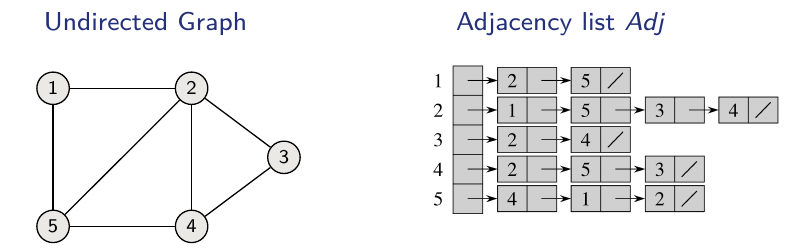
\includegraphics[scale=0.5]{images/adjacency_List}
	\caption{Representing a graph with an adjacency list}
\end{figure}
Adjacency lists are defined as :
\begin{itemize}
	\item 	An array  $Adj$ of $|V|$ lists, one per vertex (= node).
	\item 	Vertex $u$'s list has all vertices $v$ such that $(u,v) \in E$ (works for both directed and undirected graphs)
	\item 	In pseudocode, we denote the array as attribute $G.Adj$, so notation like $G.Adj[u]$ will be seen.
\end{itemize}
\subsection[BFS]{BFS : Breadth-first-Tree}
The idea here is to start with a vertex, then "send a wave", meaning you add connected elements (careful if directed) to a queue, according to the order you want (alphabet, weight, don't care,...) ; you then consider the next element in the queue, and start again. Careful : the queue is not sorted alphabetically, you go in the right order, but when considering connected vertex you add them to the queue in the chosen order.
\subsection[DFS]{DFS : Depth-first-Tree}

\subsection{Topological Sort}

\section{Flow and Cut}
You want to get as much as something (say, cheese) from a \textbf{source} (say, Gruyère) to a \textbf{sink} (say, Lausanne), through a flow network. You can transport from a point to an other (on \textbf{edges}, usually directed) some \textbf{capacity} (say, 20 cheese). Capacity from $u$ to $v$ is $c(u,v) \geq 0$

\subsection{Definition of a Flow}
A flow is a function $f: V \times V \to \R$, satisfying :
\begin{itemize}
	\item 	\textbf{Capacity constraint :} For all $u,v \in V : 0 \leq f(u,v) \leq c(u,v)$
	\item 	\textbf{Flow conservation :} For all $u \in V \setminus \{s,t\}$ :
	\[\underbrace{\sum_{v\in V} f(v,u)}_{\text{flow into }u} = \underbrace{\sum_{v\in V} f(u,v)}_{\text{flow out of }u}\]
\end{itemize}

\subsection{Ford-Fulkerson Method}
Start with 0-flow. \textbf{While} there is an augmenting path from s to t in residual network, \textbf{do} :
\begin{itemize}
	 \item 	Find augmenting path
	 \item 	Compute bottleneck = min capacity along the path
	 \item 	Increase flow on the path by the bottleneck
\end{itemize}
When finished, resulting flow is maximal


\subsection{Cut}
You can cut your network in 2 parts, $S,T$, such as $s\in S,\ t\in T$. The net flow across the cut $(S,T)$ is 
\begin{equation}
	f(S,T) = \underbrace{\sum_{u\in S,\ v\in T} f(u,v)}_{\text{flow leaving }S} - \underbrace{\sum_{u\in S,\ v\in T} f(v,u)}_{\text{Flow entering }S}
\end{equation}


\section{Data Structures for Disjoint Sets}
We want to maintain a collection $S = \{S_1,S_2,...,S_k\}$ of \uline{disjoint} dynamic\footnote{changing over time} sets. Each set is identified by a \textbf{representative}, which is some member of the set\footnote{Doesn't matter which one, we only want that, if we ask twice for a representative and no modification, we get twice the same answer}. In order to do so, we want to define 3 operations :

\texttt{Make-Set}$(x)$ :Make a new set $S_i = {x}$ and add $S_i$ to $S$.

\texttt{Union}$(x,y)$ : for $x \in S_x,\ y \in S_y \to S = S- S_x - S_y \cup \{S_x \cap S_y\}$

\texttt{Find}$(x)$ : return representative of set containing $x$.


\newpage
\appendix
\section{Proofs} \label{appendix: proofs}
\subsection{Substitution Method : Upper and lower bound}\label{appendix: substitution method}
\evid{Upper bound :} We want to prove there exists a constant $a > 0$ such that $T(n) \leq a \cdot n\log n$ for all $n \geq 2$ (and thus, $T(n) = O(n\log n)$)
\begin{itemize}
	\item 	\textbf{Base case} : For any constant $n \in \{2,3,4\},\ T(n)$ has a constant value ; if \textit{a} is larger than this value, the base case is satisfied.
	\item 	Inductive step : assume statement true $\forall n \in \{2,3,...,k-1\}$ and prove the statement for $n=k$.
	\[\begin{array}{rl}
		T(n) &= 2T(n/2) + cn\\
		&\leq 2 \cdot a \cdot \frac{n}{2} \log(n/2) + cn = a\cdot n\log(n/2) + cn\\
		&= a \cdot n\log n - \log(2)an + cn = an\log(b) - an + cn\\
		&\leq a\cdot n\log n \qquad \text{if we select } a\geq c
	\end{array}
	\]
	We can thus select $a$ to be a positive constant so that both the base case and the inductive step holds. Hence, $T(n) = O(n\log n)$
\end{itemize}
\evid{Lower bound :} We want to prove there exists a constant $b > 0$ such that $T(n) \geq b \cdot n\log n$ for all $n \geq 0$ (and thus, $T(n) = \Omega(n\log n)$)
\begin{itemize}
	\item 	\textbf{Base case} : For $n=1$, $T(n) = c$ and $b \cdot n \log n = 0$ so the base case is satisfied for any \textit{b}
	\item 	Inductive step : assume statement true $\forall n \in \{2,3,...,k-1\}$ and prove the statement for $n=k$.
	\[\begin{array}{rl}
		T(n) &= 2T(n/2) + cn\\
		&\geq 2 \cdot b \cdot \frac{n}{2} \log(n/2) + cn = b \cdot n\log(n/2) + cn\\
		&= b \cdot n\log n - \log(2)bn + cn = bn\log(b) - bn + cn\\
		&\geq b\cdot n\log n \qquad \text{if we select } b \geq c
	\end{array}
	\]
	We can thus select $b$ to be a positive constant so that both the base case and the inductive step holds. Hence, $T(n) = \Theta(n\log n)$
\end{itemize}
\newpage
\begin{thebibliography}{10}
	\bibitem{reference book} Thomas Cormen, Charles Leiserson, Ronald Rivest, Clifford Stein: Introduction to algorithms, Third Edition, MIT Press, 2009.
\end{thebibliography}
\end{document}  